\chapter{Технология кросс-архитектурной миграции}

\section{Верхнеуровневая архитектура}

\textit{1.5 страницы}

\begin{figure}[h]
\center{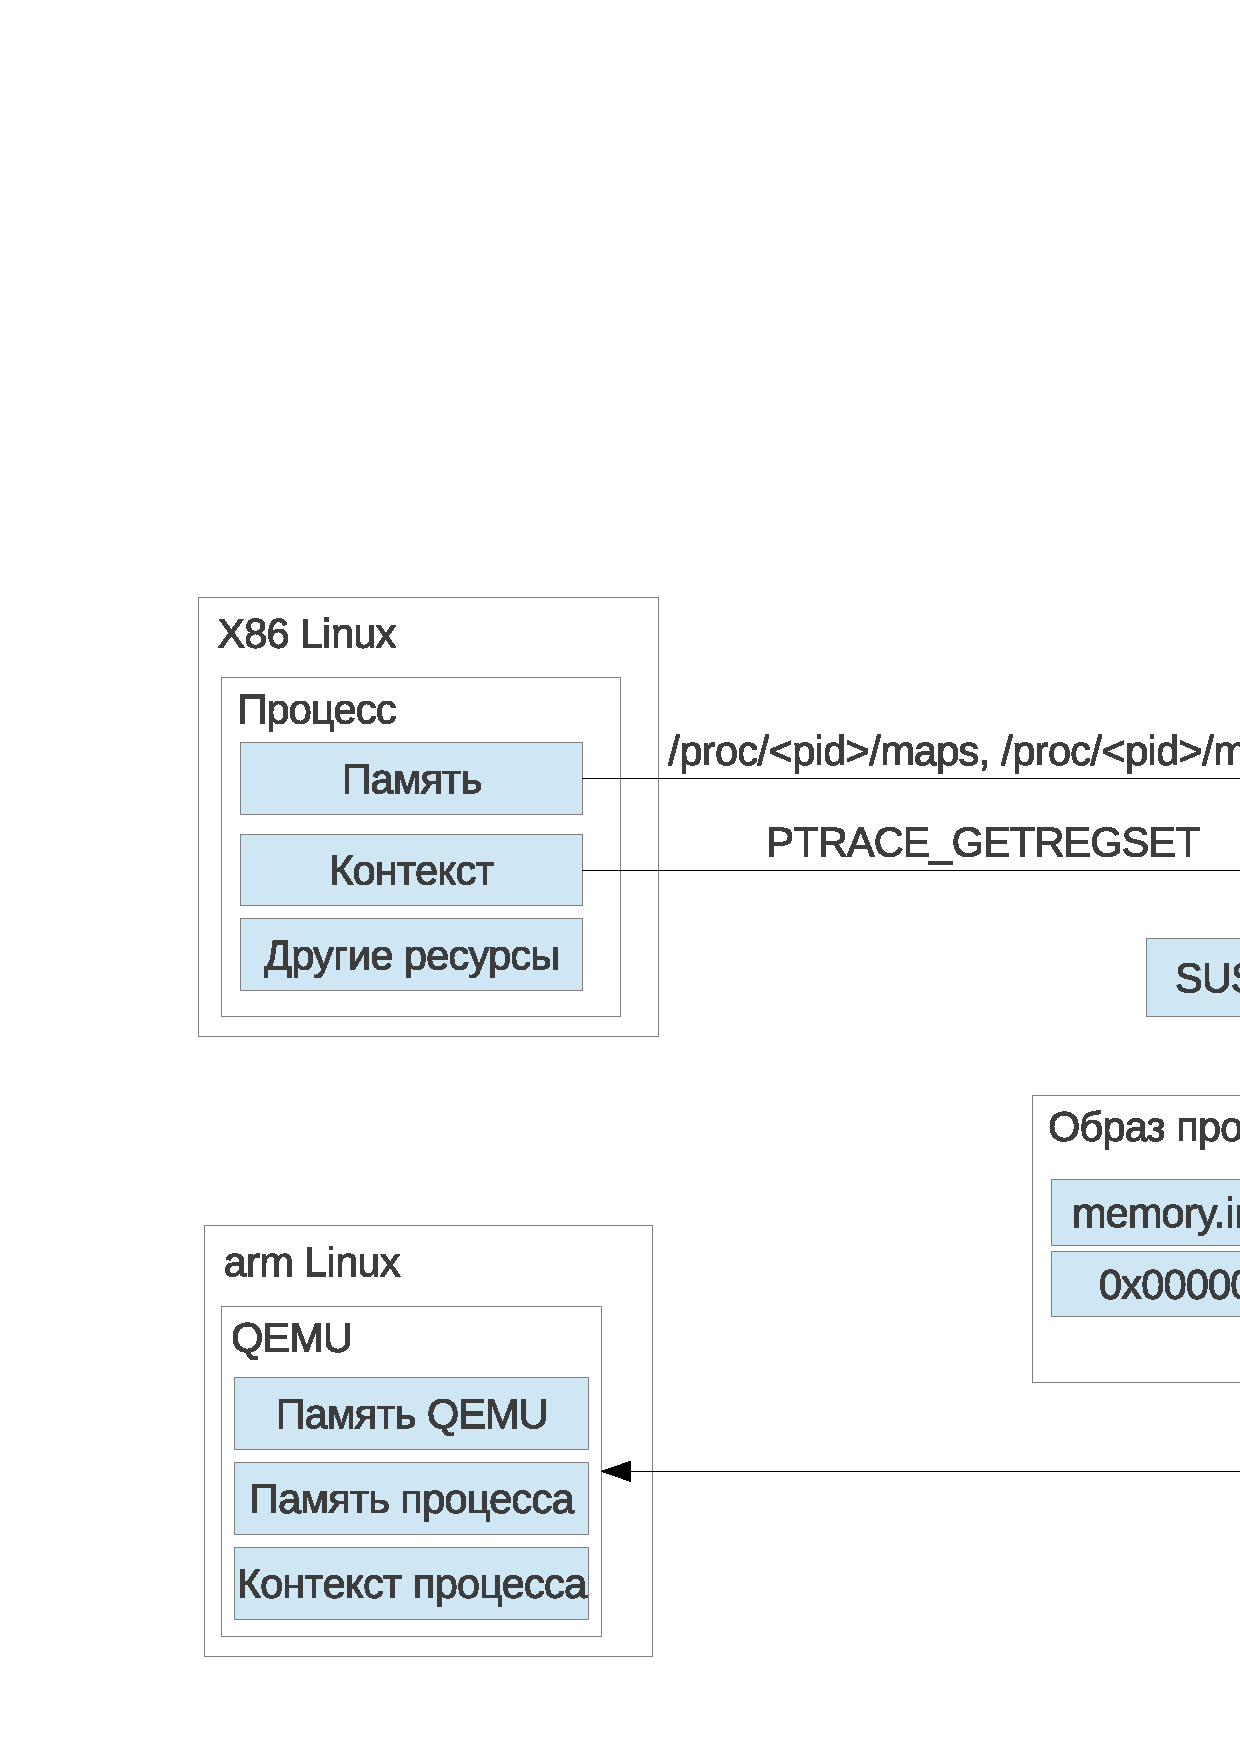
\includegraphics[width=1\linewidth]{common_arch}}
\caption{Верхнеуровневая архитектура}
\label{pic:common_arch}
\end{figure}

На рис.~\ref{pic:common_arch} изображены основные компоненты системы.

\textbf{\textit{SUSPEND Tool.}} Задача приложения собрать информацию о процессе и сохранить ее в виде набора файлов. В данной работе рассматриваются только два ресурса процесса - состояние регистров и состояние памяти.

Для доступа к информации о процессе используются интерфейсы ОС Linux - системный вызов ptrace и файловая система proc (в частности два файла maps и mem).

\textbf{\textit{QEMU.}} В качестве динамического транслятора выступает QEMU. В данной работе я внес изменения в QEMU User Mode, чтобы он мог читать файлы образа процесса и востанавливать процесс в точке останова.

Для восстановления процесса необходимо зарезервировать область под память гостевого процесса и заполнить ее содержимым памяти из образа прцесса, а также заполнить значениями из образа поля вирутального окружения QEMU.

\textbf{\textit{Формат хранения данных.}} Для описания формата хранения данных используется Protobuf~\footnote{https://code.google.com/p/protobuf/}, который позволяет по описание формата сгенрировать сгенерировать код разбора и сохранения описанной структуры.

Описание контекста сохраняется в файле registers.img, описание регионов памяти сохраняется в файле memory.img, кроме того для каждого региона памяти выделен отдельный файл, хранящий непосредственно содержимое региона памяти.

\section{Останов процесса}

\subsection{Архитектура}

\textit{1 страница}

\begin{figure}[h]
\center{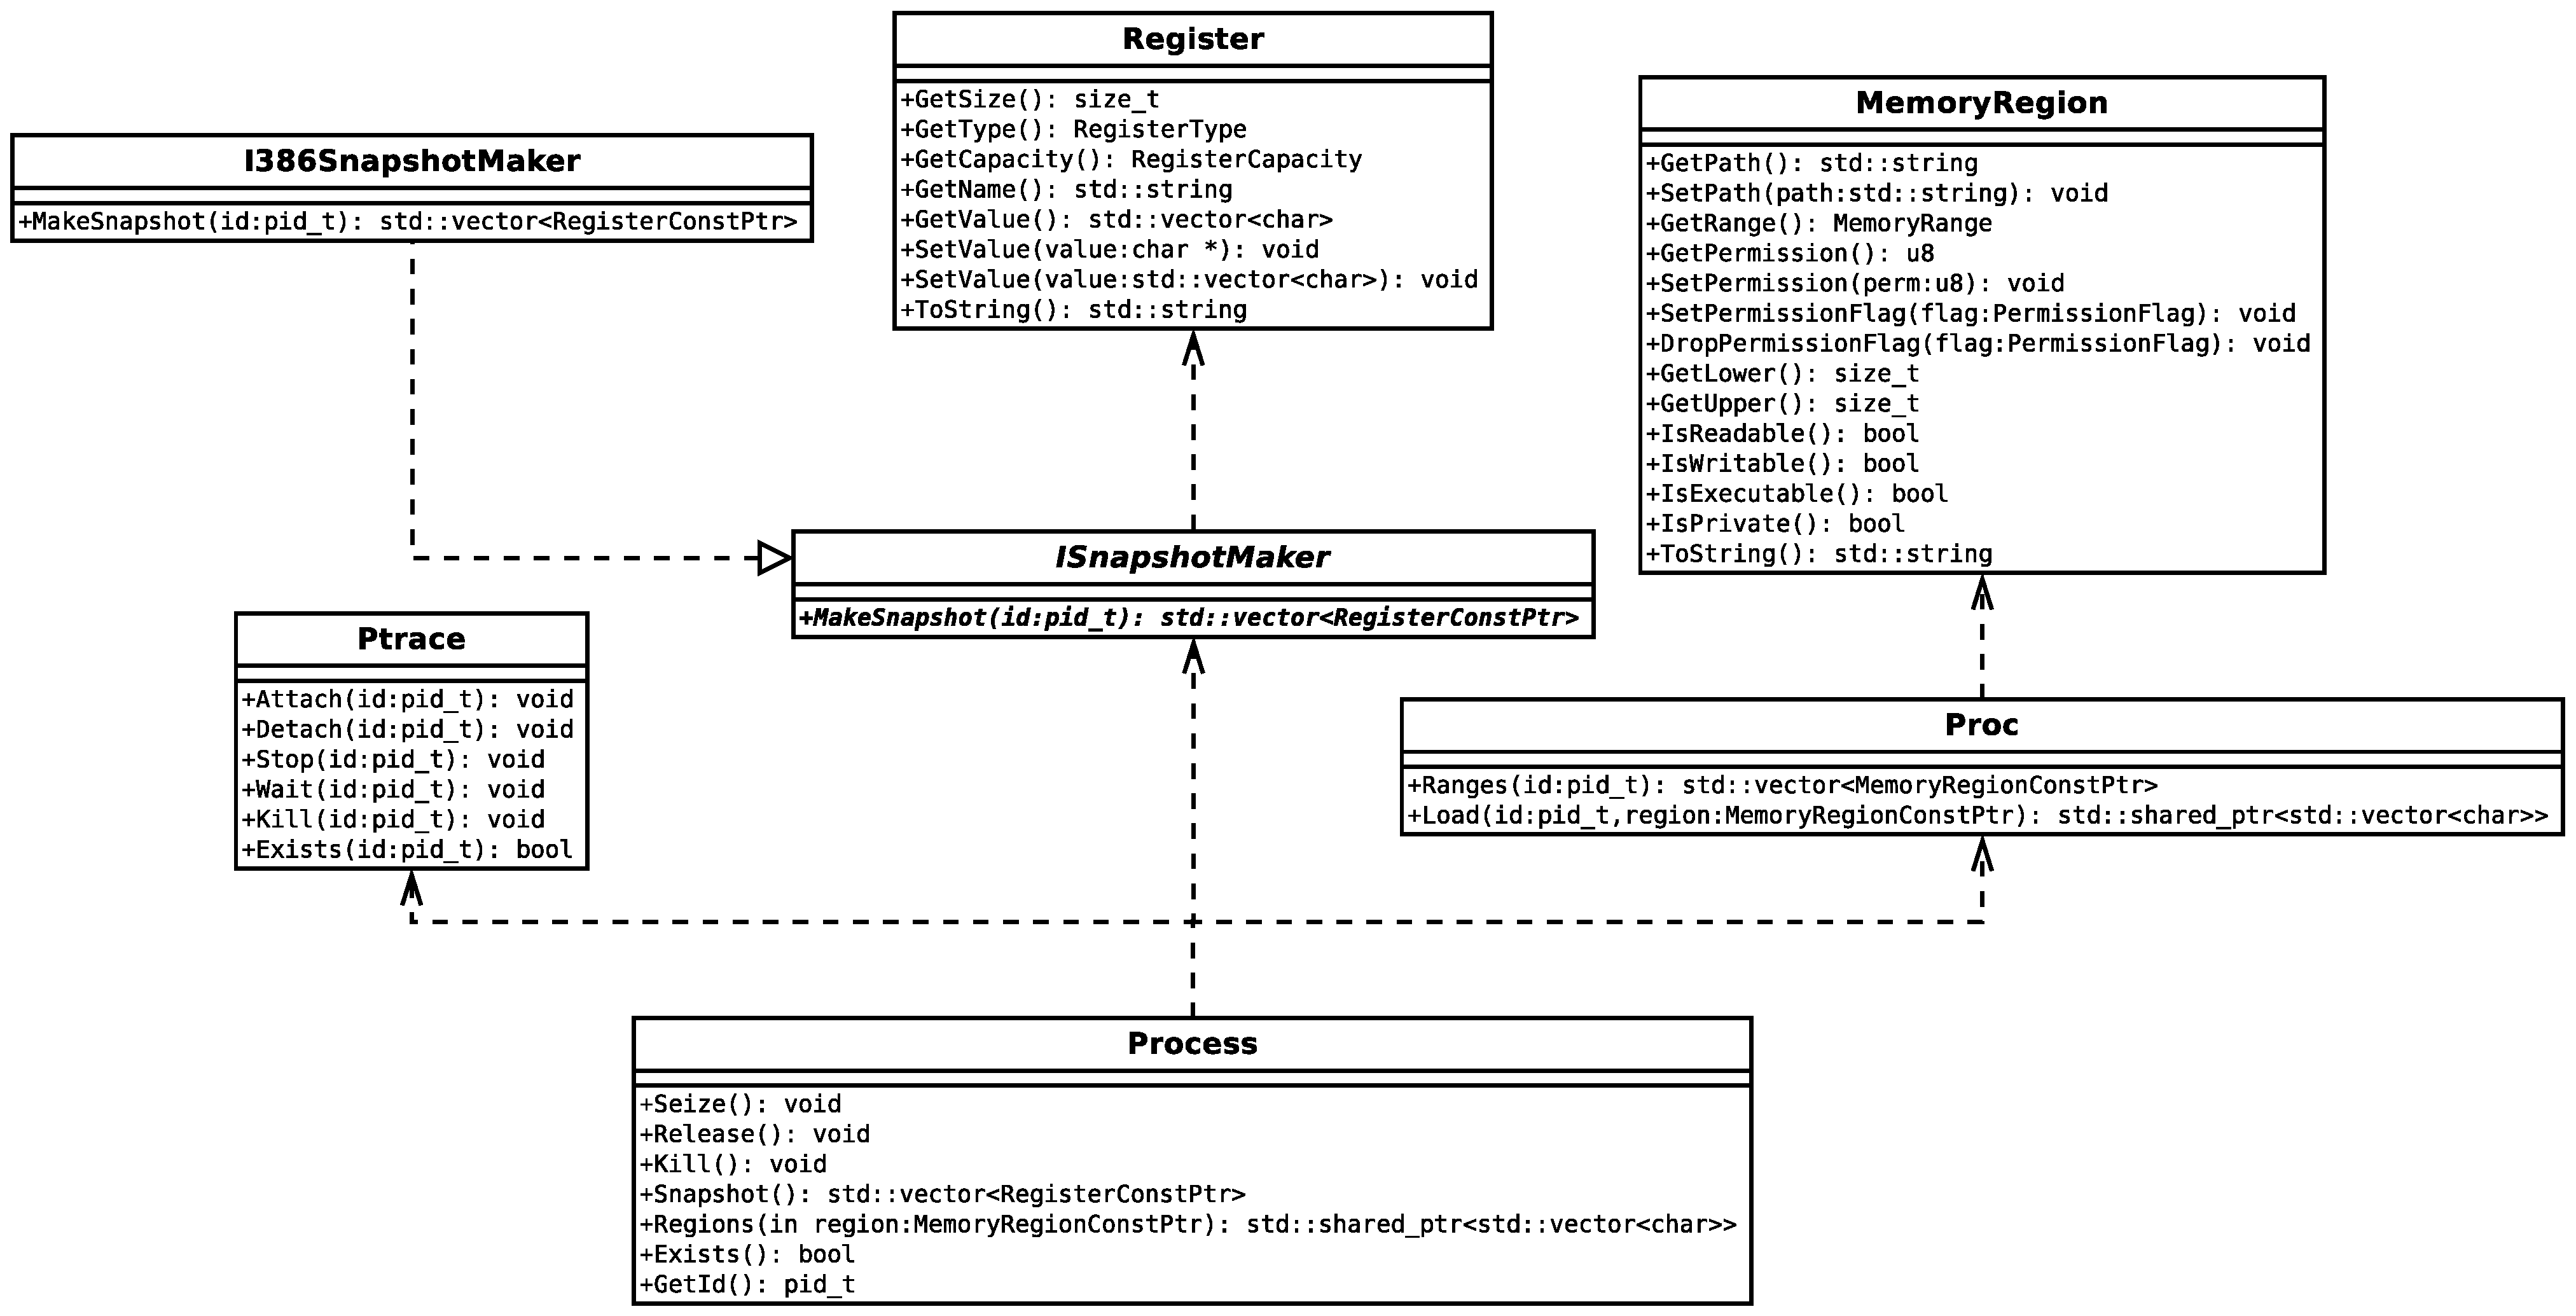
\includegraphics[width=1\linewidth]{suspend_arch}}
\caption{Рахитектура утилиты создания образа процесса}
\label{pic:suspend_arch}
\end{figure}

На рис.~\ref{pic:suspend_arch} представлены главные компоненты приложения для создания образа процесса.

\textbf{\textit{Process.}} Абстракция процесса - класс предоставляющий единый архитектурно-независимый интерфейс для захвата и останова процесса, а таже для получения его ресурсов. Класс Process зависит от трех компонентов: ptrace, proc и ISnapshotMaker.

\textbf{\textit{Ptrace.}} Обертка над системным вызовом ptrace, она предоставляет интерфейс к независимым от архитектуры коммандам ptrace.

\textbf{\textit{Proc.}} Интерфейс к файловой системе proc, для получения информации о памяти процесса.

\textbf{\textit{ISnapshotMaker.}} Контекст исполнения процесса получается с помощью системного вызова ptrace, однако набор регистров отличен для различных платформ, поэтому получение состояния регистров выделено в отдельный интерфейс. Задача ISnapshotMaker сделать снимок регистров и привести его к архитектурно независимому виду.

Чтобы поддержать другую аппаратную платформу в приложении (например, arm), потребуется реализовать интерфейс ISnapshotMaker и зарегистрировать его с помощью макроса DECLARE\_IMPLEMENTATION.

\subsection{Системный вызов ptrace}

Системный вызов ptrace предоставляет широкие возможности по отслеживанию состояния процесса, а также позволяет изменять состояние процесса прямо во время работы, эту возможность, например, активно использует дебагер gdb. В библиотеке glibc существует обертка для доступа к ptrace (см. листинг~\ref{code:ptrace})

\begin{lstlisting}[caption=Вызов ptrace, label=code:ptrace]
    #include <sys/ptrace.h>
    long ptrace(enum __ptrace_request request, pid_t pid, void *addr, void *data);
\end{lstlisting}

В литинге~\ref{code:ptrace}:

\begin{itemize}

    \item request - номер команды для выполнения
    \item pid - id целевого процесса
    \item addr - значение зависит от комманды, как правило, обозначает адрес в адресном пространстве целевого процесса
    \item data - указатель на данные, в которых хранится (или сохраняется в результате вызова ptrace), конкретный тип данных зависит от команды.

\end{itemize}

В данной работе ptrace используется для захвата и останова процесса, а также для получения снимка регистров процесса.

\textbf{\textit{Захват процесса.}} Для захвата процесса существуют следующие команды ptrace: PTRACE\_TRACEME, PTRACE\_ATTACH.

\begin{itemize}

    \item PTRACE\_TRACEME - после этой команды родительский процесс может наблюдать за процессом из которого был произведен вызов. Типичное использование - запуск приложения под отладчиком, когда отладчик после того как сделал fork и перед загрузкой целевого приложения в память исполняет комманду PTRACE\_TRACEME, таким образом захватывая целевой процесс.

    \item PTRACE\_ATTACH - позволяет произвольному процессу подключаться к любому другому процессу, pid которого передается в параметре pid. Для исполнения этой комманды процесс должен быть запущен с правами суперпользователя.

\end{itemize}

\textbf{\textit{Останов процесса.}} Для останова процесса используется команда PTRACE\_INTERRUPT. Надо отметить, что это не единственная команда позволяющая остановить процесс, но в отличие от команды PTRACE\_STOP или команд остановки по условию она не создает дополнительных побочных эффектов (например, посылки сигналов или каких-либо других эффектов влияющих на работу целевого процесса).

\textbf{\textit{Получение списка регистров.}} Для получения списка регистров используется команда PTRACE\_GETREGSET. В аргументе addr передается константа описывающие набор регистров (например, константа NT\_PRSTATUS используется для получения "основного" набора регистров, а константа NT\_PRFPREG для получения регистров FPU).

\begin{lstlisting}[caption=Основной набор регистров, label=code:general]
    struct user_regs_struct32 {
        __u32 ebx, ecx, edx, esi, edi, ebp, eax;
        unsigned short ds, __ds, es, __es;
        unsigned short fs, __fs, gs, __gs;
        __u32 orig_eax, eip;
        unsigned short cs, __cs;
        __u32 eflags, esp;
        unsigned short ss, __ss;
    };
\end{lstlisting}

Основной набор регистров, который используется в работе описывается структурой из листинга~\ref{code:general}. Для представления регистров в программе используется класс Register (см. рис.~\ref{pic:arch}). Преобразованием структуры из листинга~\ref{code:general} в вектор объектов класса Register занимается класс I386SnapshotMaker реализующий интерфейс ISnapshotMaker.

\begin{lstlisting}[caption=Формат сохранения регистров, label=code:regs_proto]
    package protobuf;

    message Register {
        required string name = 1;
        enum Type {
            INTEGER = 0;
            FLOATING_POINT = 1;
        }
        required Type type = 2;
        enum Capacity {
            BIT8 = 8;
            BIT16 = 16;
            BIT32 = 32;
            BIT64 = 64;
            BIT128 = 128;
        }
        required Capacity capacity = 3;
        required bytes value = 4;
    }

    message RegistersSnapshot {
        repeated Register register = 1;
    }
\end{lstlisting}

Формат сохранения состояния регистров определеяется файлом описания protobuf из листинга~\ref{code:regs_proto}. Код сохранения и чтения генерируется с помощью компилятора protoc во время сборки проекта.

\subsection{Файловая система proc}

\begin{lstlisting}[caption=Формат файла maps, label=code:maps]
08048000-08057000 r-xp 00000000 08:03 5899468    /usr/bin/update-notifier

...

08863000-08bae000 rw-p 00000000 00:00 0          [heap]
41000000-41020000 r-xp 00000000 08:03 5636122    /lib/i386-linux-gnu/ld-2.15.so
41020000-41021000 r--p 0001f000 08:03 5636122    /lib/i386-linux-gnu/ld-2.15.so

...

411ca000-411cb000 rw-p 001a5000 08:03 5636768    /lib/i386-linux-gnu/libc-2.15.so
411cb000-411ce000 rw-p 00000000 00:00 0 
4342d000-43527000 r-xp 00000000 08:03 5636775    /lib/i386-linux-gnu/libglib-2.0.so.0.3400.1
43527000-43528000 r--p 000f9000 08:03 5636775    /lib/i386-linux-gnu/libglib-2.0.so.0.3400.1

...

b77e6000-b77e8000 rw-p 00000000 00:00 0 
b77e8000-b77e9000 r-xp 00000000 00:00 0          [vdso]
bfc44000-bfc65000 rw-p 00000000 00:00 0          [stack]
\end{lstlisting}

proc - виртуальная файловая система предоставляющая информацию о процессах. Каждому процессу в файловой системе proc соответсвует директория /proc/<pid>, где <pid> - id процесса. В работе я использую файловую систему proc для доступа к памяти процесса.

Внутри ядра Linux информация о каждом регионе памяти процесса хранится в структуре vm\_area\_struct, все регионы объединены в список упорядоченный по начальному адресу региона, указатель на голову списка хранится в структуре mm\_struct в поле mmap (см. листинг~\ref{code:mm_struct}). В пространстве пользователя доступ к этой информации может быть осуществлен через файл maps, который имеет формат представленный в листинге~\ref{code:maps}: 

\begin{enumerate}

    \item столбец содержит адреса занимаемые регионом памяти [начальный; конечный).

    \item столбец описывает права региона памяти:

        \begin{itemize}

            \item r (read) - регион доступен для чтения
            \item w (write) - регион доступен для записи
            \item x (execute) - регион может содержать исполянемый код
            \item p (private) - регион приватный, т. е. не разделяется с другими процессами

        \end{itemize}

    \item стобец описывает смещение в файле, если регион - файл отображенный в память, и содержит 0 в противном случае.

    \item столбец содрежит минорный и мажоный номер устройства, на котором находится файл, если регион - отображенный в память файл.

    \item столбец содержит inode соответствующий отображенному файлу и 0 в противном случае

    \item столбцец содержит путь к отображенному файлу или назначение региона памяти (например, [heap] или [stack]).

\end{enumerate}

По каждой строке файла maps создается описатель региона памяти MemoryRegion (см. рис.~\ref{pic:common_arch}). Описатели всех регионов памяти сохраняются в файл memory.img. Формат файла описывается файлом protbuf из листинга~\ref{code:maps_proto}.

\begin{lstlisting}[caption=Формат сохранения описателей регионов памяти, label=code:maps_proto]
    package protobuf;

    message MemoryRegion {
        required uint64 lower = 1;
        required uint64 upper = 2;
        required string path = 3;

        required bool readable = 4;
        required bool writable = 5;
        required bool executable = 6;
        required bool shared = 7;
    }

    message MemoryRegions {
        repeated MemoryRegion region = 1;
    }
\end{lstlisting}

Непосредственно память процесса доступна через файл mem. Байту со смещением x в адресном пространстве процесса соответствует байт со смещением x в файле mem. Попытка доступа к файлу со смещением не попадающим не в один из регионов памяти приводит к ошибке. Так как целевой процесс может занимать много памяти, содержимое регионов памяти загружается по требованию, после чего сразу же сохраняется в соответсвующий файл на диске, а память освобождается.

\subsection{Организация проекта и система сборки}

Конфигурация проетка и сборка осуществляется посредством системы CMake~\footnote{http://www.cmake.org/}. Организация директорий представлена в листинге~\ref{code:dirs}

\begin{lstlisting}[caption=Организация каталогов, label=code:dirs]
    +- inc/ +- process/ +- {memory.h, process.h, registers.h, serialize.h}
    |       |           |
    |       |           +- proc/ +- proc.h
    |       |           |
    |       |           +- ptrace/ +- ptrace.h, snapshot.h
    |       |                      |
    |       |                      +- i386/ +- snapshot.h
    |       |
    |       +- utils/ +- {casts.h, exceptions.h, range.h, string_utils.h, types.h}
    |       |
    |       +- i386/ +- types.h
    |
    +- src/ +- core/ +- main.cpp
            |
            +- lib/ +- serialize.cpp
            |       |
            |       +- process/ +- proc/ +- proc.cpp
            |                   |
            |                   +- ptrace/ +- ptrace.cpp
            |                              |
            |                              +- i386/ +- snapshot.cpp
            |
            +- protobuf/ +- {memory.proto, snapshot.proto}
            |
            +- test/ +- {casts.cpp,  protobuf.cpp, registers.cpp, string_utils.cpp}
\end{lstlisting}

Проект имеет следующие зависимости

\begin{itemize}

    \item Boost unit\_test\_framework
    \item Boost program\_options
    \item Boost regex
    \item Protobuf

\end{itemize}

\begin{lstlisting}[caption=Генерация исходных кодов по файлам описания protobuf, label=code:custom_command]
set(PROTO_SRC ${MANTICORE_LIBRARY_DIR}/snapshot.pb.cc ${MANTICORE_LIBRARY_DIR}/memory.pb.cc)
set(PROTO_HDR ${MANTICORE_LIBRARY_DIR}/snapshot.pb.h ${MANTICORE_LIBRARY_DIR}/memory.pb.h)
list(APPEND PROTO_FILES_ALL ${PROTO_HDR})
list(APPEND PROTO_FILES_ALL ${PROTO_SRC})
add_custom_target(protogen)
add_custom_command(
	TARGET protogen
	COMMAND protoc
	ARGS -I=${MANTICORE_PROTOBUF_DIR} --cpp_out=${MANTICORE_LIBRARY_DIR} ${MANTICORE_PROTOBUF_DIR}/snapshot.proto
)
add_custom_command(
	TARGET protogen
	COMMAND protoc
	ARGS -I=${MANTICORE_PROTOBUF_DIR} --cpp_out=${MANTICORE_LIBRARY_DIR} ${MANTICORE_PROTOBUF_DIR}/memory.proto
)
message(STATUS "GENERATED SOURCES: " ${PROTO_FILES_ALL})
set_source_files_properties(${PROTO_FILES_ALL} PROPERTIES GENERATED TRUE)
\end{lstlisting}

Для генерации файлов C++ по файлам описания protobuf используется метод add\_custom\_command CMake, как описано листинге~\ref{code:custom_command}.

Все исходные коды утилиты создания образа процесса находятся в свободном доступе~\footnote{https://github.com/OSLL/manticore}.

\section{Восстановление процесса}

\subsection{Организация QEMU и система сборки}

\textit{1 страница}

Основные компоненты транслятора QEMU. User Mode режим.

\subsection{Восстановление памяти гостевого процесса}

\textit{1 страница}

Отображение адресов гостя в адреса хоста (картинка). Проблема нехватки адресного пространства и ее "решение". Интерфейсы QEMU для резервирования памяти. Чтение файлов protobuf.

\subsection{Восстановление регистров процессора}

\textit{0.5 страницы}

Виртуальный процессор QEMU (вырезка из структуры). Чтение файлов protobuf.
